%
% 卒論レジュメフォーマット Ver.2.0 pLaTeX版
%
\documentclass[twocolumn]{jarticle} % 2段組のスタイルを用いている

\usepackage{wuse_resume}
\usepackage{url}	% \url{}コマンド用.URLを表示する際に便利
\usepackage[dvipdfmx]{graphicx}  % ←graphicx.styを用いてEPSを取り込む場合有効にする
			% 他のパッケージ・スタイルを使う場合には適宜追加

%%%%%%%%%%%%%%%%%%%%%%%%%%%%%%%%%%%%%%%%%%%%%%%%%%%%%%%%%%%%%%%%%%%%%%%%

%%
%% タイトル,学生番号,氏名などを設定する
%%

\タイトル{ScratchにおいてCTスキルが向上するリミックス作品の分析}
\研究室{ソーシャルソフトウェア工学}
\学生番号{60266269}
\氏名{堀尾 桃夏}

\概要{%
本研究では,Scratchにおける作品推薦に有効な情報と基準を明確化するために,リミックス作品の分析を行う.Scratchとは,命令処理を持つブロックを直観的に操作し,プログラミングを行うビジュアルプログラミング言語である.公開作品を編集することをリミックスという.従来研究で,リミックスにより使用するブロックの種類数とCTスキルが向上することが分かった.極端な難易度のものをリミックスしてもCTスキルへの効果が少なく,ユーザのCTスキルに寄与したものは,ユーザのCTスキルに適した作品のリミックスだと考える.しかし,Scratchにはキーワード検索に限るため,ユーザのCTスキルに適した作品を探すことは困難である.ユーザのCTスキルに適したリミックス元作品の推薦が有効であり,そのためには推薦に有効な情報と基準が求められる.本研究では,リミックス前後のCTスコアの差分を取得し,リミックス作品とユーザのCTスキルの関係を分析する. 
}

\キーワード{プログラミング教育}
\キーワード{Scratch}
\キーワード{コンピュテーショナル・シンキング}
\キーワード{作品分析}
\キーワード{ユーザ分析}

%%%%%%%%%%%%%%%%%%%%%%%%%%%%%%%%%%%%%%%%%%%%%%%%%%%%%%%%%%%%%%%%%%%%%%%%

%% 以下の3行は変更しない

\begin{document}
\maketitle
\thispagestyle{empty} % タイトルを出力したページにもページ番号を付けない

%%%%%%%%%%%%%%%%%%%%%%%%%%%%%%%%%%%%%%%%%%%%%%%%%%%%%%%%%%%%%%%%%%%%%%%%

%%
%% 本文 - ここから
%%

\section{はじめに}
アメリカでは,Scratch\cite{resnick2009scratch}と呼ばれるプログラミング初学者向けのビジュアルプログラミング言語を通してプログラミング教育を行っている.Scratchでは命令処理をもつブロックを組み合せて作品を完成させる.また,作品はオンライン上に公開することができ,公開されている他ユーザの作品を複製し,編集することも可能である.この機能をリミックスという.

Scratchにおいて,ユーザが作品のCTスキルを計測するためには,作品評価ツールであるDr.Scratch\cite{moreno2015dr}を使用する.Dr.Scratchとは,Morenoらによって開発されたScratch作品評価ツールであり,作品の評価を7概念に基づいて行う.また,CTスキルの各概念を0点から3点の,合計21点とする.

従来研究でYangら\cite{10.1145/2724660.2724674}と橋谷ら\cite{橋谷直樹2022scratch}により,リミックスを行うことでCTスキルが向上することが示された.寄与したものは,ユーザのCTスキルに適した難易度の作品のリミックスだと考える.ユーザのCTスキルに適した難易度の作品を探す手段として,リミックス元作品の推薦が有効である.推薦のためにはCTスキル向上に有効な作品の情報と基準が求められる.

本研究では,Scratchのリミックス機能におけるユーザのCTスキルに適した作品推薦に向けて,ユーザのCTスキルとリミックス作品の関係について分析を行う.具体的には,以下の3つのReseach Question(RQ)に対して回答する.
\begin{itemize}
  \item{RQ1:CTスコアは他ユーザの作品をリミックスすることによって向上するか?}
  \item{RQ2:リミックスにより向上しやすいCTスキルの概念は異なるか?}
  \item{RQ3:CTスコアによって,向上しやすいCTスキルの概念は異なるか?}
\end{itemize}

\section{RQ1:CTスコアは他ユーザの作品をリミックスすることによって向上するか?}
\subsection{分析手法}
本研究では,リミックス前作品,リミックス元作品,リミックス作品,リミックス後作品を重視する.
\begin{itemize}
  \item リミックス前作品:リミックス以前のオリジナル作品で,CTスコアが最も高い作品.

  \item リミックス後作品:リミックス以降のオリジナル作品3件で,CTスコアが最も高い作品.

\end{itemize}
CTスコアに基づき,リミックス元作品とリミックス前作品のスコア差とリミックス前後の作品を比較し,向上,低下したユーザ数により分析する.

\subsection{分析結果・考察}
%-------------------
\begin{figure}[h]
\centerline{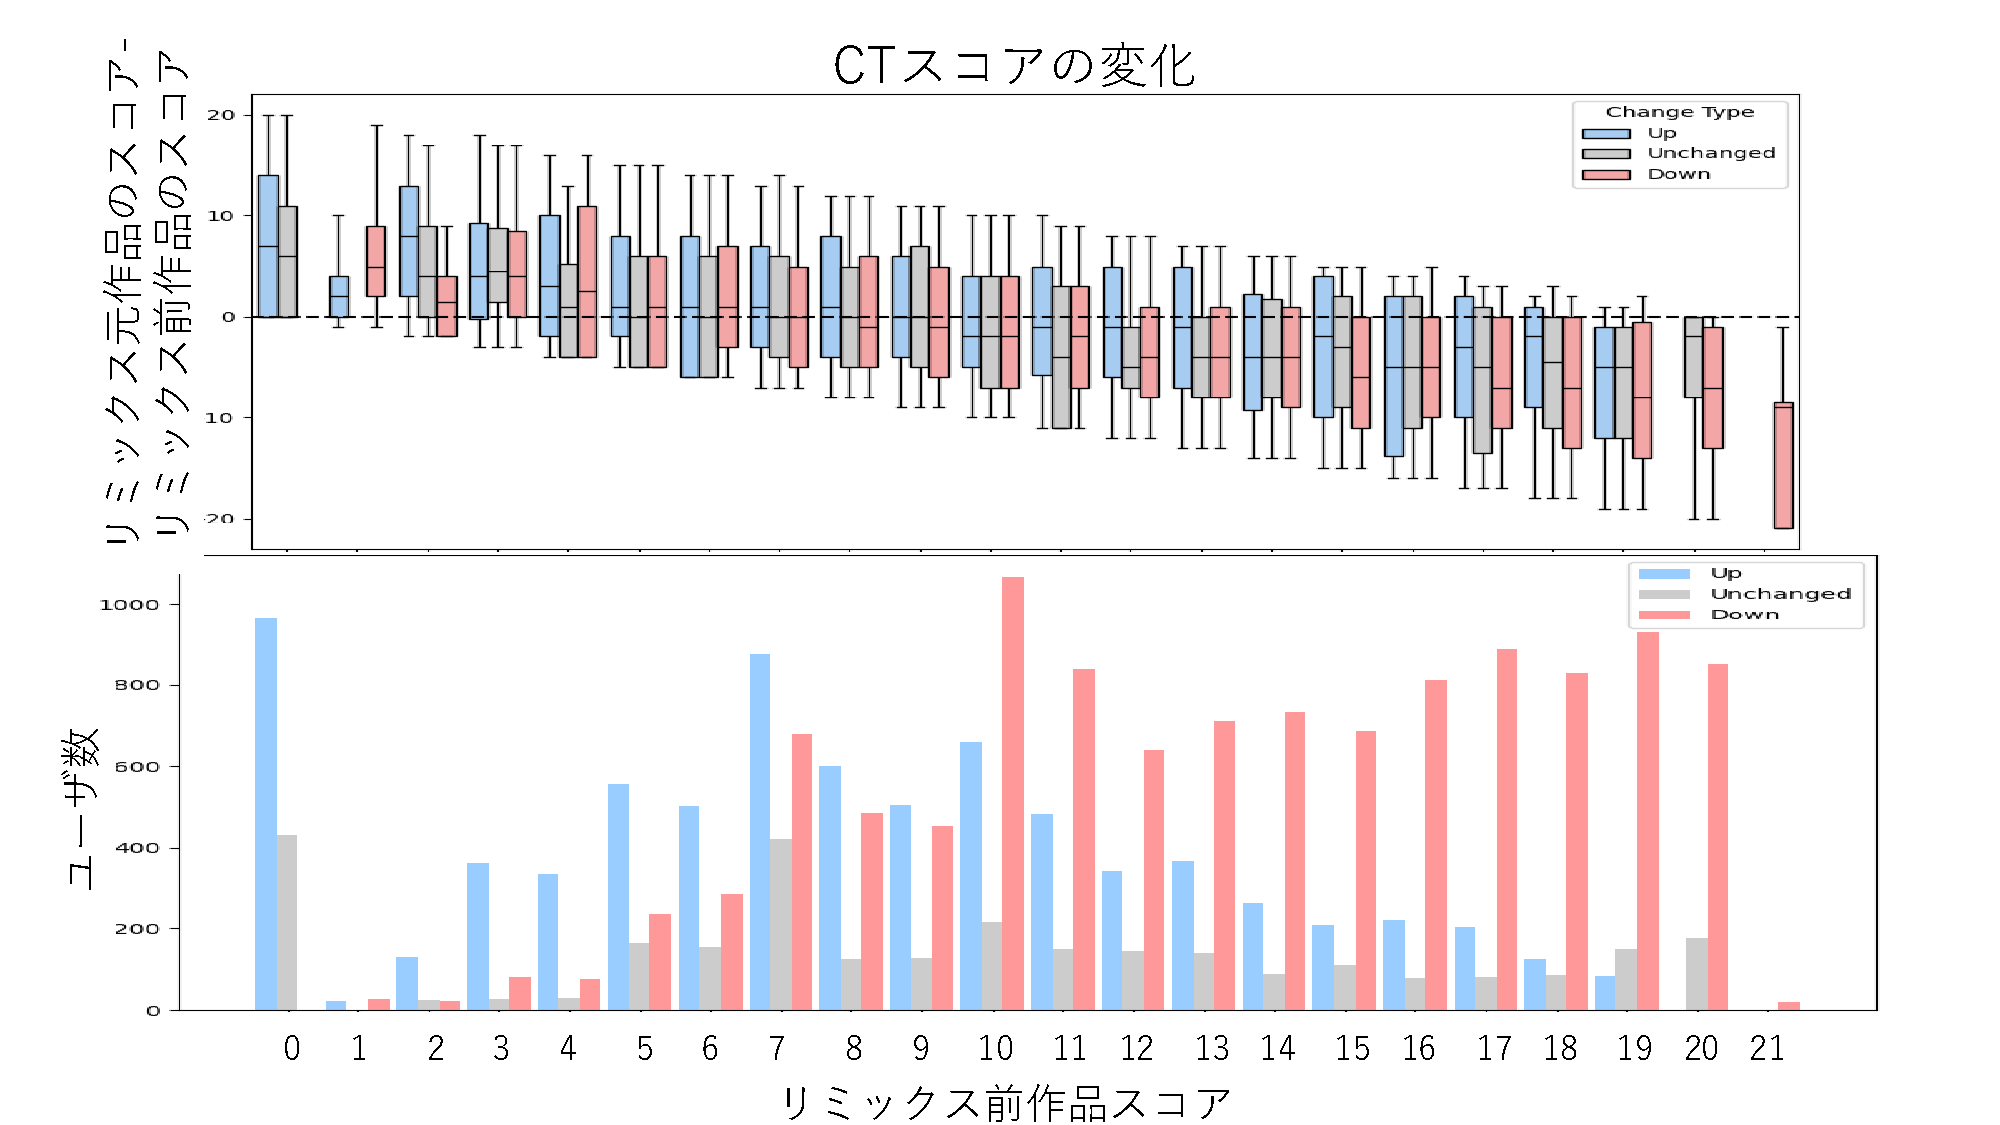
\includegraphics[width=1.0\linewidth]{@BSthesis2024_Horio/BSthesis2024_Horio_fig/resume_rq1.pdf}}
\caption{リミックスによるCTスコア変化}
\label{fig:}
\end{figure}
%-------------------

9点以下は向上したユーザ数が低下したユーザ数を上回っており,10点以上は低下したユーザ数が向上したユーザ数を上回っていることから,リミックスはCTスコアが9点以下のユーザに対し有効であり,10点以上のユーザに対しては効果が少ない.また,向上したユーザが低下したユーザに比べてCTスコアが高い作品も低い作品もリミックスしている.このことから,リミックス元作品とユーザのCTスコア差はCTスコア向上に大きな影響を与えず,どの作品をリミックスしても効果が得られると考えられる.

\section{RQ2:リミックスにより向上しやすいCTスキルの概念は異なるか?}
\subsection{分析手法}
CTスキルの各概念に基づき,リミックス元作品とリミックス前作品のスコア差と,リミックス前後の作品を比較し,向上,低下したユーザ数により分析する.
\subsection{分析結果・考察}
%-------------------
\begin{figure}[h]
\centerline{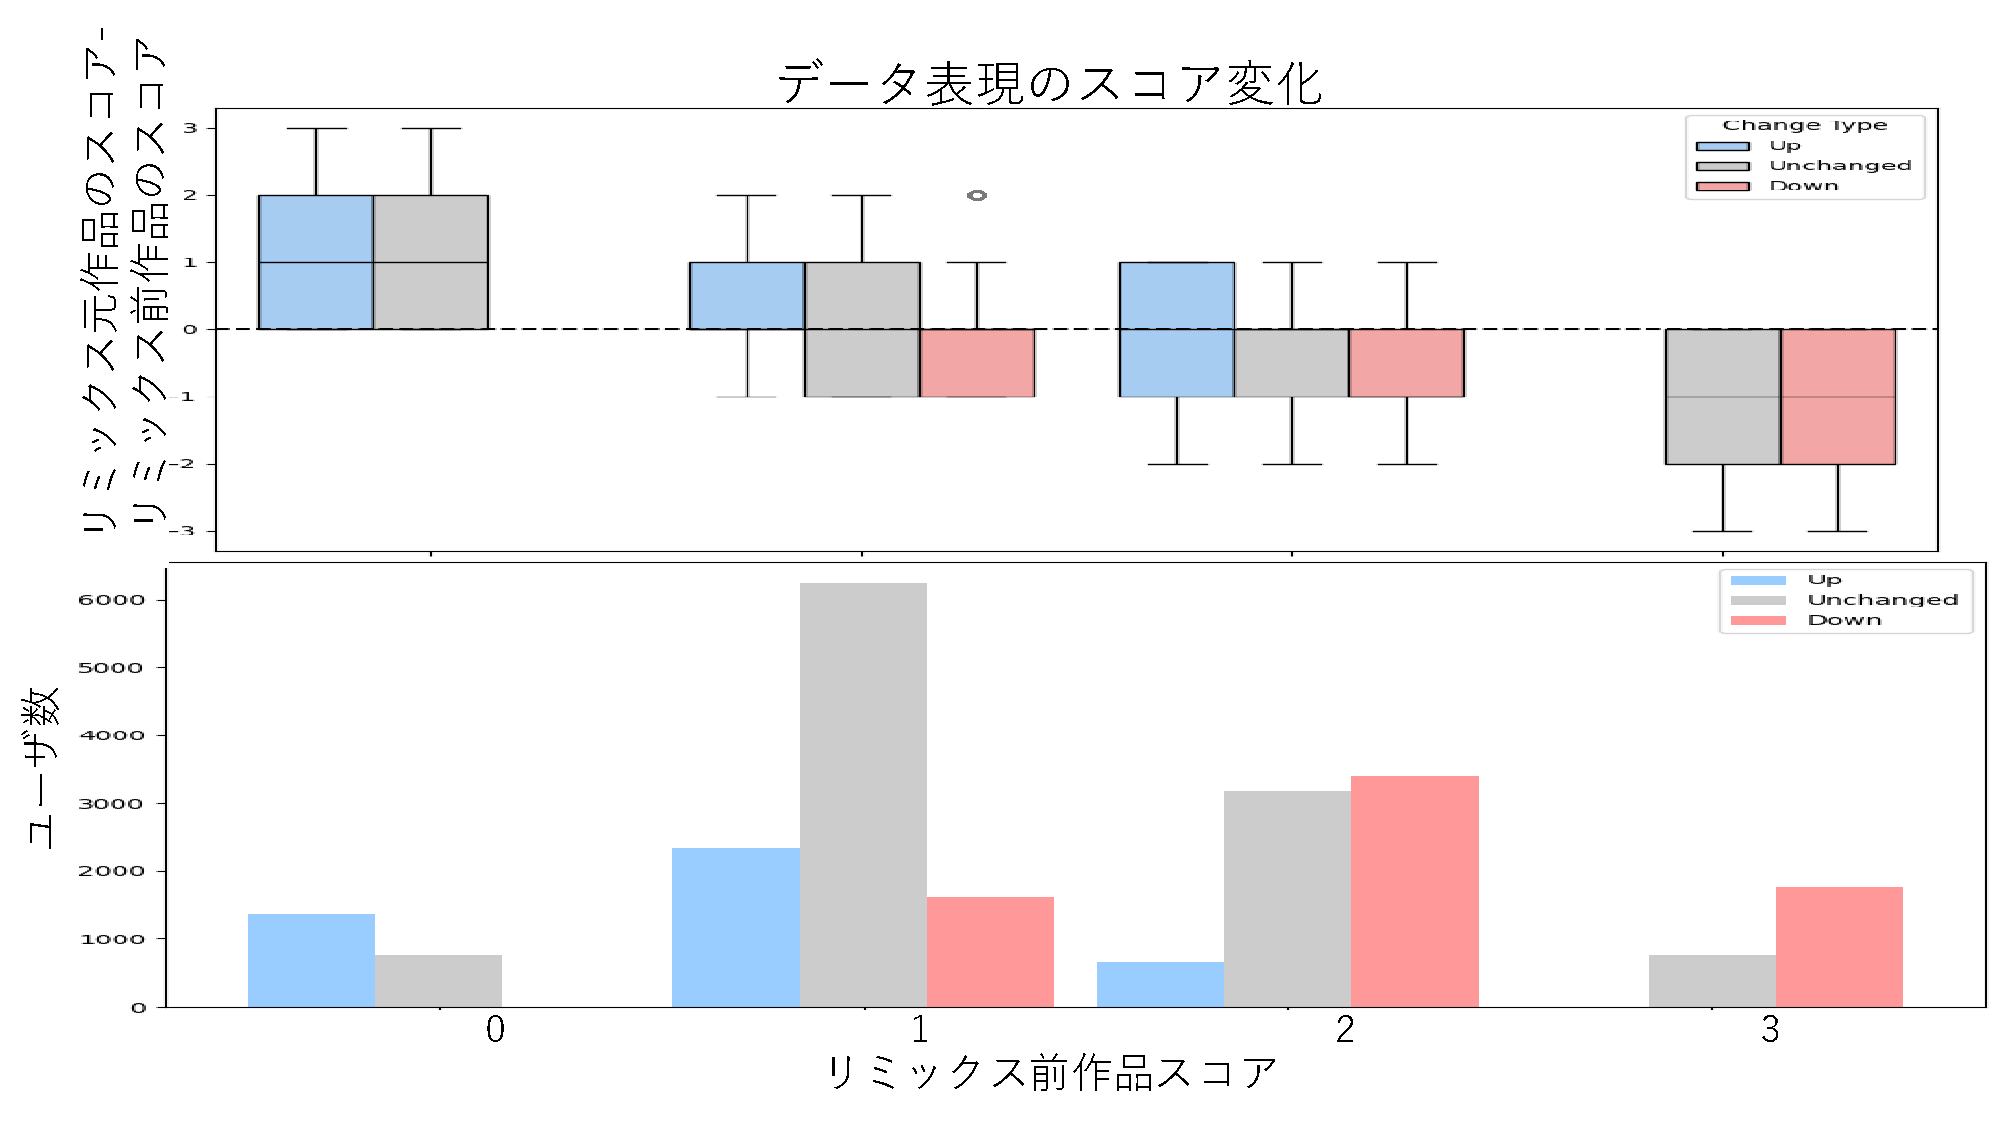
\includegraphics[width=0.8\linewidth]{@BSthesis2024_Horio/BSthesis2024_Horio_fig/resume_rq2.pdf}}
\caption{リミックスによるデータ表現のスコア変化}
\label{fig:}
\end{figure}
%-------------------
並列や論理では,向上したユーザと低下したユーザのリミックス元作品のスコアに差がなく,リミックス元作品とユーザのスコア差はスコア向上に大きな影響を与えず,どの作品をリミックスしても効果が得られる可能性がある.
向上したユーザと低下したユーザのリミックス元作品のスコア差があるものとして.抽象化,データ表現,ユーザ対話性が挙げられる.向上したユーザはリミックス元作品のスコアが高く,スコアがユーザより高い作品をリミックスすると効果が得られる.特に,データ表現,ユーザ対話性では,1点以下のユーザがユーザのスコアより高い作品をリミックスをすることで効果が得られやすい.
リミックスによって向上しやすいCTスキルの概念が異なるだけでなく,CTスキルの各概念のスコアによっても,向上のしやすさに違いがあることがわかる.

\section{RQ3:CTスコアによって,向上しやすいCTスキルの概念は異なるか?}
\subsection{分析手法}
CTスコアにおけるCTスキルの各概念に基づき,リミックス元作品とリミックス前作品のスコア差と,リミックス前後の作品を比較し,向上,低下したユーザ数により分析する.
\subsection{分析結果・考察}
%-------------------
\begin{figure}[h]
\centerline{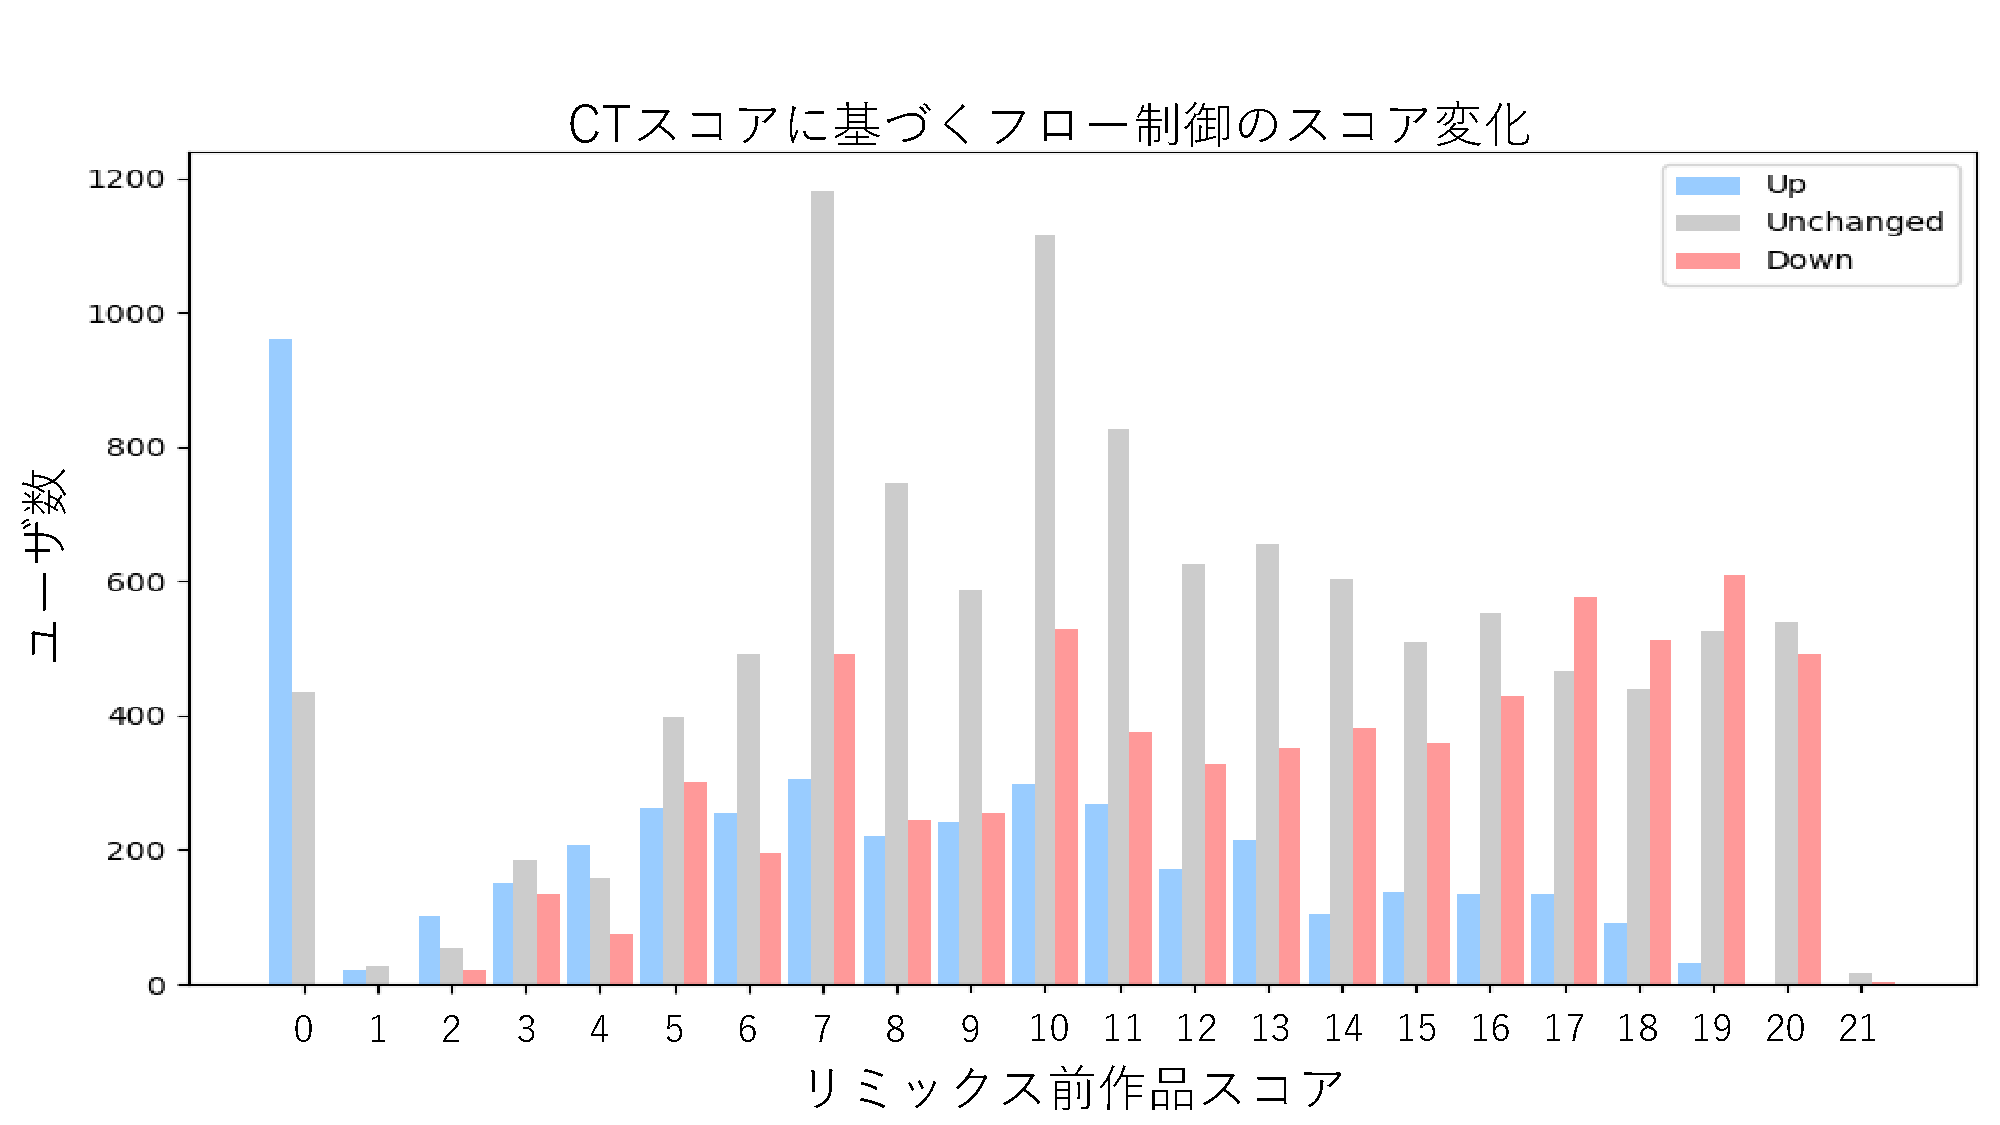
\includegraphics[width=0.8\linewidth]{@BSthesis2024_Horio/BSthesis2024_Horio_fig/resume_rq3.pdf}}
\caption{CTスコアに基づくフロー制御のスコア変化}
\label{fig:}
\end{figure}
%-------------------
抽象化,フロー制御では,向上したユーザ数が低下したユーザ数に比べて一度下回っているが,スコアが上がると,向上したユーザ数と低下したユーザ数に大差がなくなっている.これは,スコアを向上させるために必要なCTスキルの他概念が不足しており,CTスコアが上がった際に十分になった可能性がある.このことから,CTスキルの各概念には相関関係があることが考えられる.

\section{おわりに}
本研究では,Scratchのリミックス機能におけるユーザのCTスキルに適した作品推薦に向けて,分析を行った.今後は,CTスキルの各概念の相関関係を明らかにすることで,スコア向上に有効な作品が明確になると考える.


%%
%% 本文 - ここまで
%%

%%%%%%%%%%%%%%%%%%%%%%%%%%%%%%%%%%%%%%%%%%%%%%%%%%%%%%%%%%%%%%%%%%%%%%%%

%%
%% 参考文献
%%
\bibliographystyle{junsrt}
\bibliography{@BSthesis2024_Horio/BSthesis2024_Horio}

%%%%%%%%%%%%%%%%%%%%%%%%%%%%%%%%%%%%%%%%%%%%%%%%%%%%%%%%%%%%%%%%%%%%%%%%

\end{document}
